\title{Coordinate Systems}
\subtitle{\SubTitleName}
\institute[]{\Course}
\author{\Instructor}
\maketitle  


\frame{\frametitle{Topics and Objectives}
\Emph{Topics} \\
\TopicStatement
\begin{itemize}
    \item change of basis
    \item coordinates relative to a basis
    % \item dimension of a subspace
    % \item the rank of a matrix 
\end{itemize}

\vspace{0.5cm}

\Emph{Objectives}\\

\LearningObjectiveStatement

\begin{itemize}
    \item calculate the coordinates of a vector in a given basis
    % \item characterize a subspace using the concept of dimension (or cardinality)
    % \item characterize a matrix using the concepts of rank, column space, null space
    % \item apply the rank, basis, and matrix invertibility theorems to describe matrices and subspaces
\end{itemize}
 
}

\frame{\frametitle{Choice of Basis}

\Emph{Key idea:} There are many possible choices of basis for a subspace. Our choice can give us dramatically different properties.

\vspace{0.5cm}

\pause 

\Emph{Example}: sketch $\vec b_1 + \vec b_2$ for the two different coordinate systems below. 

\begin{center}
  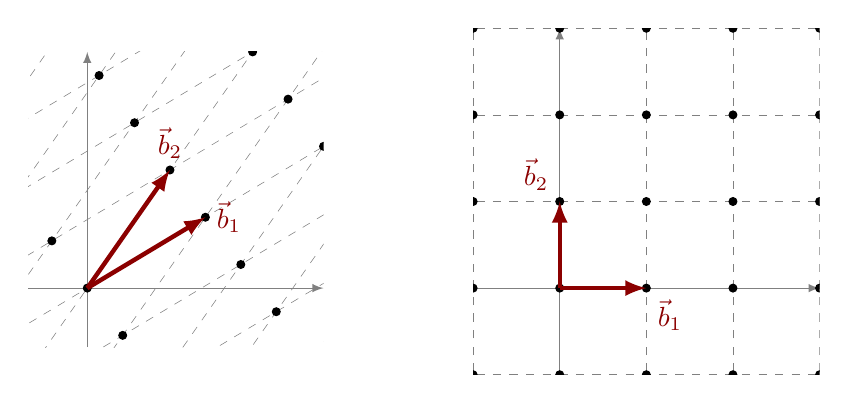
\begin{tikzpicture}

    \usetikzlibrary{calc}
    \begin{scope}[xshift=6cm, scale=1.1] 
    
    \coordinate (Origin)   at (0,0);
    \coordinate (XAxisMin) at (-1,0);
    \coordinate (XAxisMax) at (3,0);
    \coordinate (YAxisMin) at (0,-1);
    \coordinate (YAxisMax) at (0,3);
    \draw [thin, gray,-latex] (XAxisMin) -- (XAxisMax);% Draw x axis
    \draw [thin, gray,-latex] (YAxisMin) -- (YAxisMax);% Draw y axis

   \clip (-1,-1) rectangle (3,3); % Clips the picture...
%    \pgftransformcm{1}{0.6}{0.7}{1}{\pgfpoint{0cm}{0cm}}
          % This is actually the transformation matrix entries that
          % gives the slanted unit vectors. You might check it on
           % MATLAB etc. . I got it by guessing.
    \coordinate (Bone) at (0,1);
    \coordinate (Btwo) at (1,-1);
    \draw[style=help lines,dashed] (-14,-14) grid[step=1cm] (14,14);
          % Draws a grid in the new coordinates.
          %\filldraw[fill=gray, fill opacity=0.3, draw=black] (0,0) rectangle (2,2);
              % Puts the shaded rectangle
    \foreach \x in {-7,-6,...,7}{% Two indices running over each
      \foreach \y in {-7,-6,...,7}{% node on the grid we have drawn 
        \node[draw,circle,inner sep=1pt,fill] at (\x,\y) {};
            % Places a dot at those points
      }
    }
    \draw [ultra thick,-latex,DarkRed] (Origin) -- (Bone) node [above left] {$\vec b_2$};
%    \draw [ultra thick,-latex,red] (Origin) -- (Btwo) node [below right] {$2b_2$};
   \draw [ultra thick,-latex,DarkRed] (Origin) -- ($(Bone)+(Btwo)$) node [below right] {$\vec b_1$};
    %\draw [ultra thick,-latex,red] (Origin) -- ($2*(Bone)+(Btwo)$) node [above right] {$2\vec b_1+2\vec b_2$};
%    \filldraw[fill=gray, fill opacity=0.3, draw=black] (Origin) rectangle ($2*(Bone)+(Btwo)$);
    %\draw [thin,-latex,red, fill=gray, fill opacity=0.3] (0,0)
        % -- ($2*(0,2)+(2,-2)$)
        % -- ($3*(0,2)+2*(2,-2)$) -- ($(0,2)+(2,-2)$) -- cycle;
    \end{scope}

    \begin{scope}[scale=.75]
    
    \coordinate (Origin)   at (0,0);
    \coordinate (XAxisMin) at (-1,0);
    \coordinate (XAxisMax) at (4,0);
    \coordinate (YAxisMin) at (0,-1);
    \coordinate (YAxisMax) at (0,4);
    \draw [thin, gray,-latex] (XAxisMin) -- (XAxisMax);% Draw x axis
    \draw [thin, gray,-latex] (YAxisMin) -- (YAxisMax);% Draw y axis

   \clip (-1,-1) rectangle (4,4); % Clips the picture...
    \pgftransformcm{1}{0.6}{0.7}{1}{\pgfpoint{0cm}{0cm}}
          % This is actually the transformation matrix entries that
          % gives the slanted unit vectors. You might check it on
           % MATLAB etc. . I got it by guessing.
    \coordinate (Bone) at (0,2);
    \coordinate (Btwo) at (2,-2);
    \draw[style=help lines,dashed] (-14,-14) grid[step=2cm] (14,14);
          % Draws a grid in the new coordinates.
          %\filldraw[fill=gray, fill opacity=0.3, draw=black] (0,0) rectangle (2,2);
              % Puts the shaded rectangle
    \foreach \x in {-7,-6,...,7}{% Two indices running over each
      \foreach \y in {-7,-6,...,7}{% node on the grid we have drawn 
        \node[draw,circle,inner sep=1pt,fill] at (2*\x,2*\y) {};
            % Places a dot at those points
      }
    }
    \draw [ultra thick,-latex,DarkRed] (Origin)
        -- (Bone) node [above ] {$\vec b_2$};
    %\draw [ultra thick,-latex,red] (Origin) -- (Btwo) node [below right] {$b_2$};
    \draw [ultra thick,-latex,DarkRed] (Origin) -- ($(Bone)+(Btwo)$) node [ right] {$\vec b_1$};
    %\draw [ultra thick,-latex,red] (Origin) -- ($2*(Bone)+(Btwo)$) node [above left] {$\vec b_1+ \vec b_2$};
    %\filldraw[fill=gray, fill opacity=0.3, draw=black] (Origin) rectangle ($2*(Bone)+(Btwo)$);
    %\draw [thin,-latex,red, fill=gray, fill opacity=0.3] (0,0)
        % -- ($2*(0,2)+(2,-2)$)
        % -- ($3*(0,2)+2*(2,-2)$) -- ($(0,2)+(2,-2)$) -- cycle;
    \end{scope}
        
  \end{tikzpicture}

\end{center}
}

\frame{\frametitle{Definition: Coordinate Vector}

    Let $ \mathcal B = \{\vec b_1 ,\dotsc, \vec b_p\}$ be a basis for a subspace $ H$.  
    If $\vec x$ is in $H$, then \Emph{coordinates of $ \vec x$ relative $ \mathcal B$} are the weights (scalars) $ c_1 ,\dotsc, c_p$ so that 
    $$ \vec x = c_1 \vec b_1 + \cdots + c_p \vec b _p $$
    
    \pause 
    
    And 
    \begin{equation*}
    [x] _{\mathcal B} = 
    \begin{bmatrix*}[r]
    c_1 \\ \vdots \\ c_p 
    \end{bmatrix*}
    \end{equation*}
    is the \Emph{coordinate vector of $ \vec x$ relative to $ \mathcal B$}, or the \Emph{$ \mathcal B$-coordinate vector of $ \vec x$}

}

\frame{\frametitle{Example: Coordinate Vector}
    Let $ \vec v_1 = \begin{bmatrix*}[r]
    1 \\ 0 \\ 1
    \end{bmatrix*}$, 
    $ \vec v_2 = \begin{bmatrix*}[r] 1 \\ 1 \\ 1  \end{bmatrix*}$, 
    and 
    $ \vec x =\begin{bmatrix*}[r]
    5 \\ 3 \\ 5
    \end{bmatrix*}$.  Verify that $\vec  x $ is in the span of $ \mathcal B= \{\vec v_1 , \vec v_2\}$, and calculate  
    $ [\vec x] _{\mathcal B}$. 

}


\frame{\frametitle{Summary}

    \SummaryLine \vspace{4pt}
    \begin{itemize}\setlength{\itemsep}{8pt}
        \item calculating the coordinates of a vector with a given basis for a subspace
    \end{itemize}
    

}